% !TeX program = xelatex
% 基于用户指定的高中园模板。请从本目录编译。
\documentclass[aspectratio=169,10pt]{beamer}
\usepackage[UTF8,fontset=fandol]{ctex}
\IfFontExistsTF{Microsoft YaHei}{\setCJKsansfont{Microsoft YaHei}}{}
\usetheme{GaoZhongYuan}
\usepackage{amsmath,amssymb,booktabs,adjustbox}
\setbeamerfont{normal text}{size=\large}
\newcommand{\R}{\mathbb R}
\newcommand{\Z}{\mathbb Z}
\newcommand{\src}[1]{\par\vfill{\tiny\color{gray}#1}}
\newcommand{\key}[1]{\begin{block}{关键认识}#1\end{block}}
\title{3.1.1 函数的概念}
\author{高一数学}
\date{具体实例与概念应用}
\begin{document}
\campusmaketitle
\begin{frame}[t]{我们已经认识的函数}
正方形的边长为 $x$，周长为 $l$，则
\[l=4x,\qquad x>0.\]
\bigskip
\begin{enumerate}
\item 给定边长 $x=2$，周长能有几个值？
\item 它与 $y=4x\ (x\in\R)$ 是同一个函数吗？
\item $y=x$ 与 $y=\dfrac{x^2}{x}$ 是同一个函数吗？
\end{enumerate}
\src{教材第60页章引言改编。后两个问题留待本课结束回答。}
\end{frame}
\begin{frame}[t]{实例一：列车行程}
某列车以 $350\,\mathrm{km/h}$ 匀速运行半小时。\par
从这段匀速运行开始计时，路程为 $S\,\mathrm{km}$，时间为 $t\,\mathrm h$。
\[S=350t.\]
\begin{enumerate}
\item $t$ 可以取哪些值？$S$ 可以取哪些值？
\item 当 $t=0.2$ 时，$S$ 是多少？能否有两个结果？
\item 能否据此断定这段计时开始后 $1\,\mathrm h$ 行驶 $350\,\mathrm{km}$？
\end{enumerate}
\src{教材第60页问题1，措辞略作压缩。}
\end{frame}
\begin{frame}[t]{列车实例中的集合与对应}
\[A=[0,0.5],\qquad B=[0,175],\qquad S=350t.\]
\bigskip
当 $t=0.2$ 时，$S=70$，结果唯一。\par\medskip
$1\notin A$，半小时后的运动情况未知，不能由这个模型判断。
\key{先确定输入的范围，再按照对应关系寻找输出。\par
对于 $A$ 中每一个 $t$，在 $B$ 中都有唯一确定的 $S$。}
\src{教材第60页。区间包含起点和终点。}
\end{frame}
\begin{frame}[t]{实例二：工作天数与工资}
某公司按每天 $350$ 元支付工资，每周工作至少 $1$ 天、至多 $6$ 天，工作天数按整数计。
\[w=350d.\]
\begin{center}
\begin{tabular}{c|rrrrrr}
$d$（天）&1&2&3&4&5&6\\\hline
$w$（元）&350&700&1050&1400&1750&2100
\end{tabular}
\end{center}
\medskip
思考：$d$ 能否取 $0.2$？能否取 $7$？\par\medskip
列车与工资都出现“乘以 $350$”，它们是同一个函数吗？
\src{教材第61页问题2改编，明确按整数天数计。}
\end{frame}
\begin{frame}[t]{相同的式子，不同的输入范围}
\begin{align*}
\text{列车：}\quad&A_1=[0,0.5],&S&=350t,\\[8pt]
\text{工资：}\quad&A_2=\{1,2,3,4,5,6\},&w&=350d.
\end{align*}
\bigskip
输入范围不同，这两个函数不同。\par\medskip
工资的实际输出是 $\{350,700,1050,1400,1750,2100\}$。
\key{描述函数时，只有一个式子还不够。}
\src{教材第60—61页实例对比。}
\end{frame}
\begin{frame}[t]{实例三：图像也能给出对应}
\begin{columns}[T]
\begin{column}{.63\textwidth}
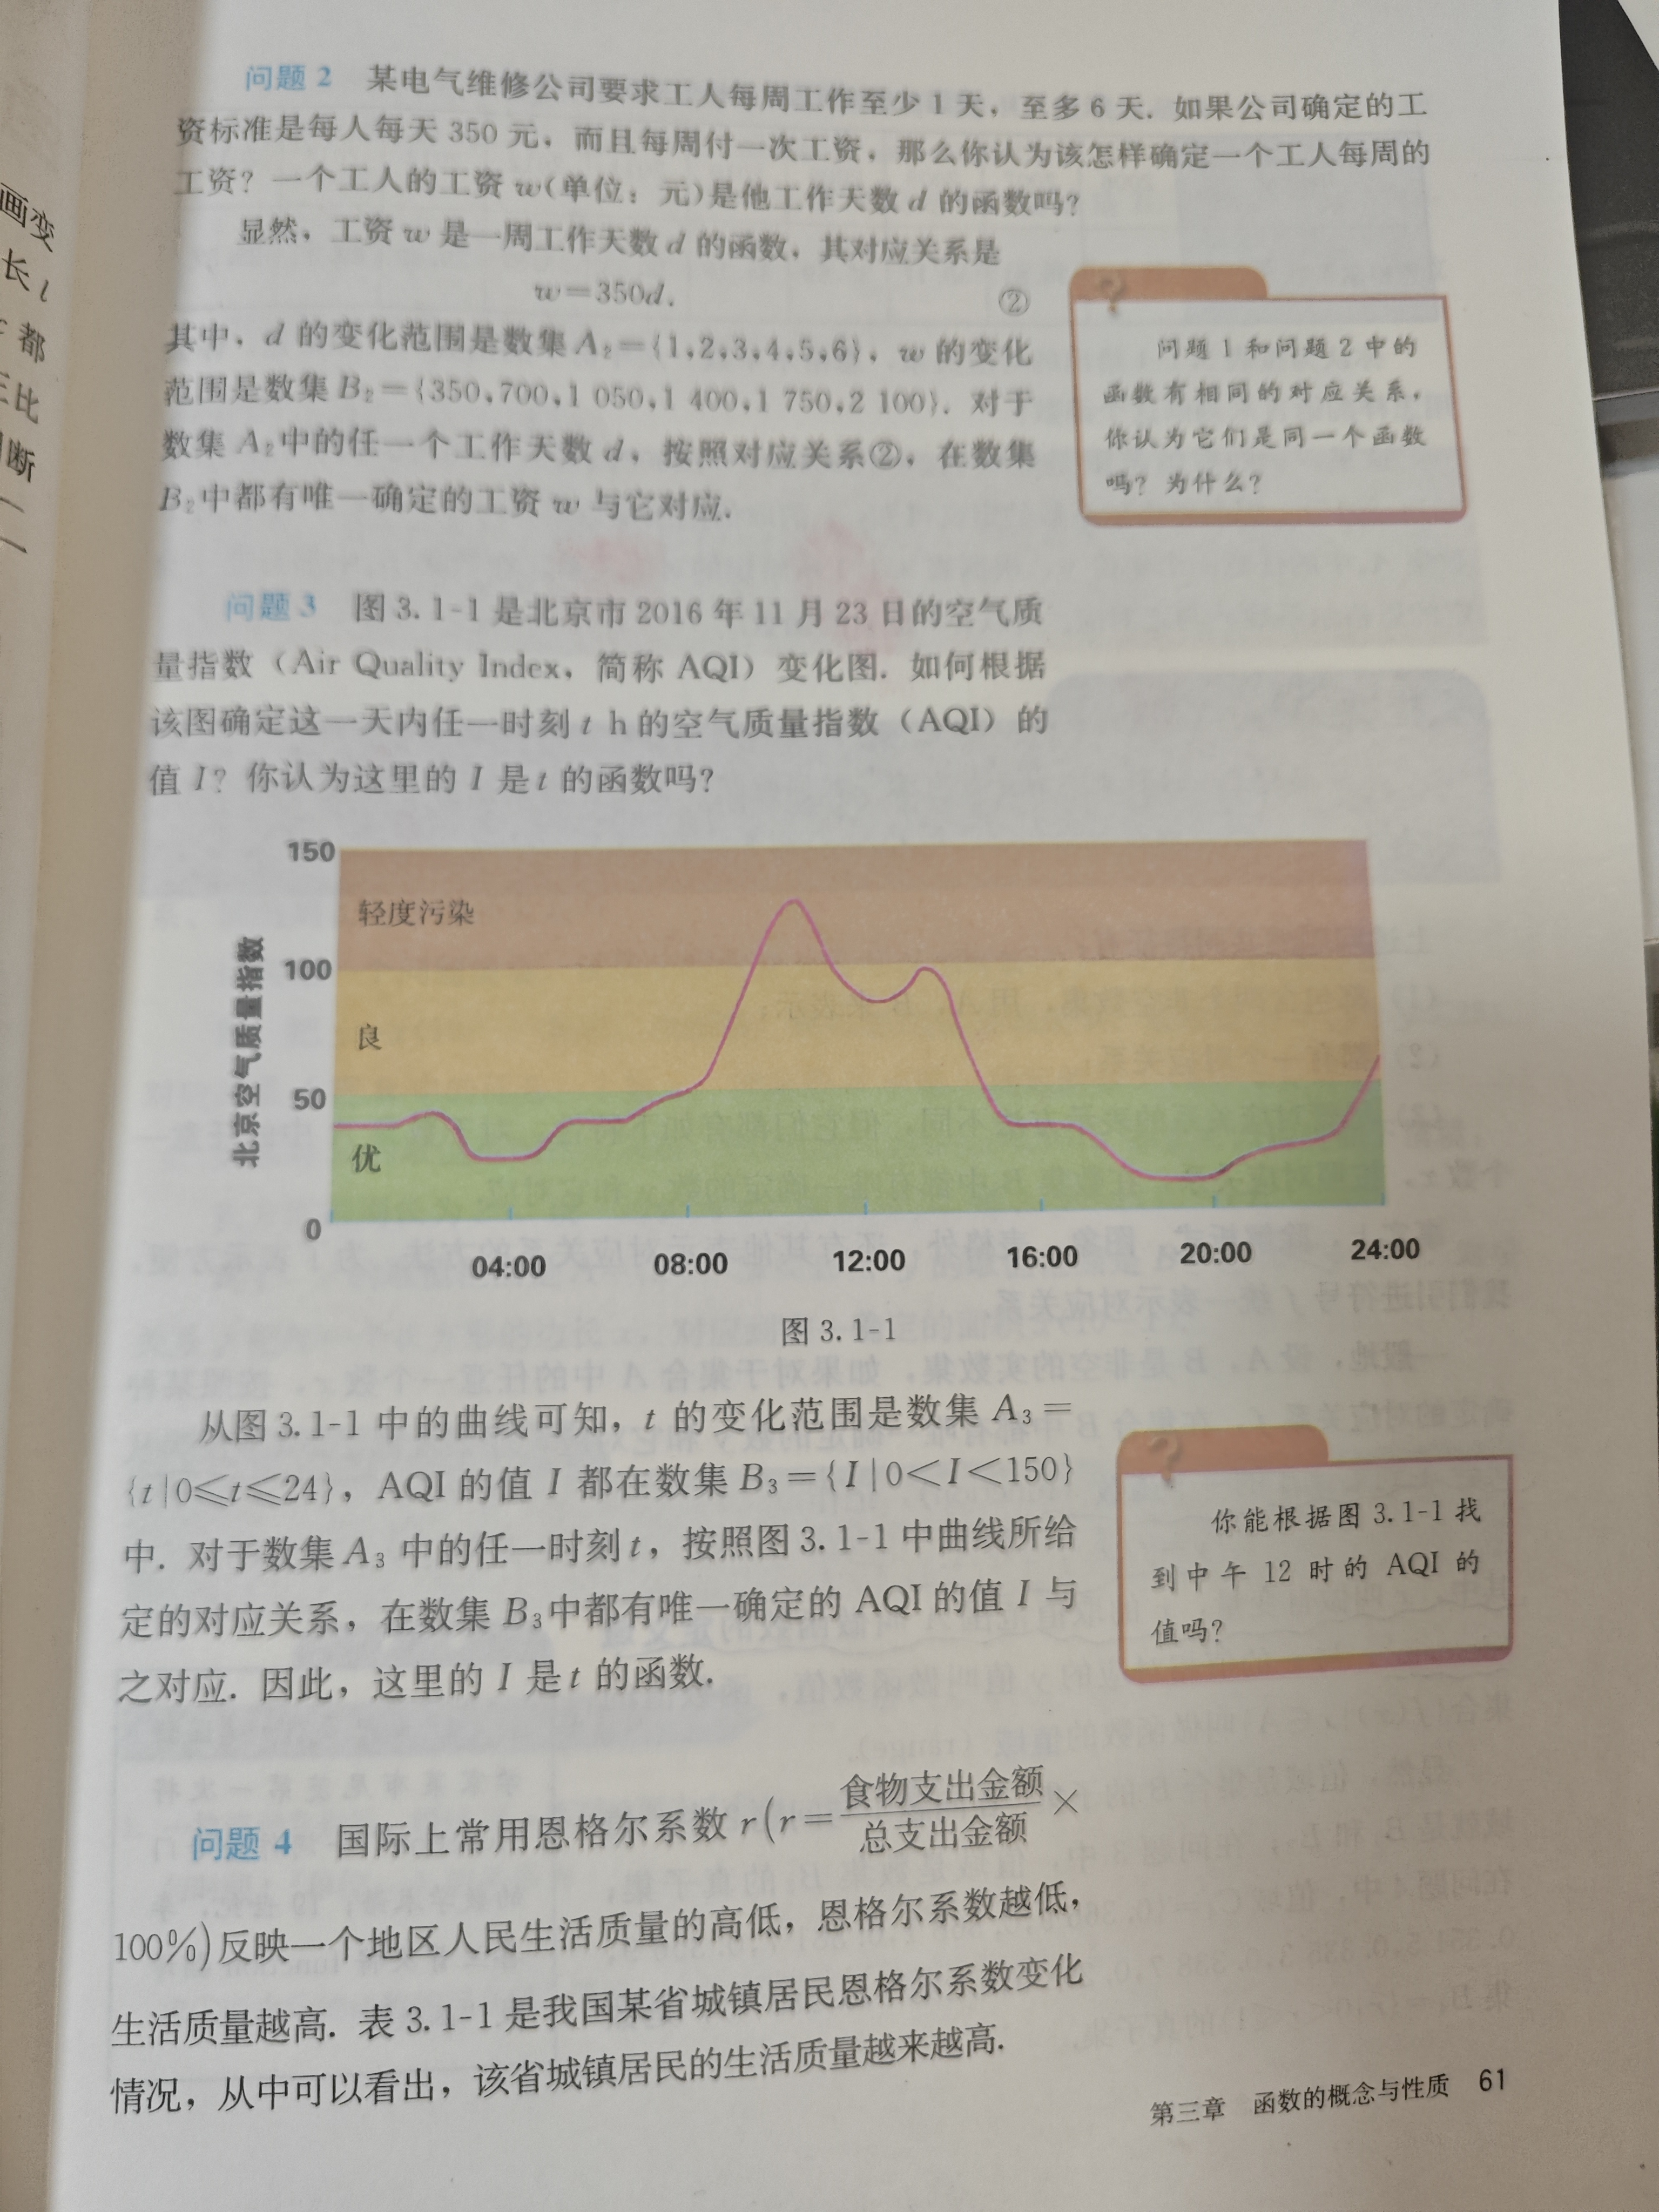
\includegraphics[trim=400bp 1600bp 430bp 1510bp,clip,width=\linewidth]{assets/教材第61页.jpg}
\end{column}
\begin{column}{.34\textwidth}
这是教材给出的某日空气质量指数图。\par\medskip
固定时刻 $t$，沿竖直方向找到曲线上的点，再读纵坐标。\par\medskip
同一时刻会读到两个不同的指数吗？
\end{column}
\end{columns}
\key{即使没有解析式，图像也能确定输入与输出的对应。}
\src{教材第61页图3.1-1原图局部。只作定性读图，不把估读值当作精确数据。}
\end{frame}
\begin{frame}[t]{实例四：表格也能给出对应}
教材列出某省城镇居民恩格尔系数：
\begin{center}\small
\begin{tabular}{c|rrrrr}
年份&2006&2007&2008&2009&2010\\\hline
系数（\%）&36.69&36.81&38.17&35.69&35.15\\\midrule
年份&2011&2012&2013&2014&2015\\\hline
系数（\%）&33.53&33.87&29.89&29.35&28.57
\end{tabular}\end{center}
\medskip
（1）2013 年对应的系数是多少？\par
（2）只根据此表，能确定 2016 年的系数吗？\par
（3）表中的每一个年份，是否都有唯一确定的系数？
\src{教材第62页表3.1-1。29.89\%=0.2989，注意百分数与小数的区别。}
\end{frame}
\begin{frame}[t]{四个实例的共同特征}
\begin{center}\small
\begin{tabular}{lll}
\toprule
实例&输入&对应关系的呈现\\\midrule
列车行程&$t\in[0,0.5]$&解析式 $S=350t$\\
工作工资&$d\in\{1,2,3,4,5,6\}$&解析式或表格\\
空气质量&$t\in[0,24]$&图像\\
恩格尔系数&表中十个年份&表格\\\bottomrule
\end{tabular}
\end{center}
\key{都有两个非空的实数集和一个确定的对应关系。\par
对输入集合中的任意一个数，输出集合中都有唯一确定的数与它对应。}
\src{教材第60—62页归纳。}
\end{frame}
\begin{frame}[t]{函数的定义}
设 $A,B$ 是\alert{非空的实数集}。如果对于集合 $A$ 中的\alert{任意一个}数 $x$，按照某种确定的对应关系 $f$，在集合 $B$ 中都有\alert{唯一确定}的数 $y$ 和它对应，\par\medskip
那么称 $f:A\to B$ 为从集合 $A$ 到集合 $B$ 的一个函数，记作
\[\boxed{y=f(x),\quad x\in A.}\]
\medskip
“任意一个”：$A$ 中的输入不能遗漏。\par
“唯一确定”：同一输入不能对应两个不同的输出。
\src{教材第62页函数定义。$f(x)$ 表示函数值，不是 $f$ 与 $x$ 相乘。}
\end{frame}
\begin{frame}[t]{定义域、函数值与值域}
取 $A=\{-1,0,1\}$，$B=\{0,1,2\}$，$f(x)=x^2$。
\[f(-1)=1,\qquad f(0)=0,\qquad f(1)=1.\]
\begin{itemize}
\item 定义域：允许输入的全部数，$A=\{-1,0,1\}$。
\item 函数值：某个输入对应的输出，例如 $f(-1)=1$。
\item 值域：实际输出的全部数，$\{0,1\}$。
\end{itemize}
\key{值域 $\{f(x)\mid x\in A\}\subseteq B$，不一定等于 $B$。\par
不同的输入可以有相同的输出。}
\src{依据教材定义自编。}
\end{frame}
\begin{frame}[t]{概念辨析：这些说法对吗？}
\begin{enumerate}
\item 一个函数必须有解析式。
\item 不同的 $x$ 必须对应不同的 $y$。
\item 集合 $B$ 中每一个数都必须被对应到。
\item $y=0\ (x\in\R)$ 也是函数。
\end{enumerate}
\bigskip
请用刚才的实例或一个反例说明理由。
\src{依据函数定义自编。}
\end{frame}
\begin{frame}[t]{概念辨析：理由比结论更重要}
\begin{enumerate}
\item 错。图像、表格也可以确定对应关系。
\item 错。$f(x)=x^2$ 中，$f(-1)=f(1)=1$。
\item 错。上例中 $2\in B$，但没有输入对应到 $2$。
\item 对。每一个实数 $x$ 都对应唯一的 $0$。
\end{enumerate}
\key{允许“多对一”，也允许常函数。\par
判断的出发点始终是定义域中的每一个输入。}
\end{frame}
\begin{frame}[t]{练习一：是否构成函数}
判断下列对应是否为从集合 $A$ 到集合 $B$ 的函数，并说明理由。
\begin{enumerate}
\item $A=\R,\ B=\{y\mid y>0\},\quad x\mapsto |x|$。
\item $A=\Z,\ B=\Z,\quad x\mapsto x^2$。
\item $A=\Z,\ B=\Z,\quad x\mapsto \sqrt{x}$。
\item $A=[-1,1],\ B=\{0\},\quad x\mapsto 0$。
\end{enumerate}
\src{《三维设计》必修第一册第31页典例1。}
\end{frame}
\begin{frame}[t]{练习一：逐个检查输入}
\begin{enumerate}
\item 不是。$0\in A$，但 $|0|=0\notin B$。
\item 是。任意整数的平方仍是唯一确定的整数。
\item 不是。$-1\in A$，却没有实数平方根。\par
即使取 $x=2$，$\sqrt2$ 也不属于 $B=\Z$。
\item 是。每一个 $x\in[-1,1]$ 都对应唯一的 $0$。
\end{enumerate}
\key{每个输入都有输出，输出属于 $B$，而且输出唯一。}
\end{frame}
\begin{frame}[t]{练习二：式子背后的定义域}
求下列函数的定义域。
\begin{enumerate}
\item $f(x)=3-\dfrac12x$。
\item $f(x)=\dfrac{(x+1)^0}{\sqrt{x+2}}$。
\item $f(x)=\dfrac{\sqrt{5-x}}{|x|-3}$。
\item $f(x)=\dfrac{\sqrt{x+1}}{\sqrt{-x^2-3x+4}}$。
\end{enumerate}
\src{《三维设计》第31页典例2。按高中实数运算约定，零次幂的底数不能为0。}
\end{frame}
\begin{frame}[t]{练习二：前两题解析}
（1）一次式对任意实数都有意义，定义域为 $\R$。\par\bigskip
（2）各部分必须同时有意义：
\[\begin{cases}x+1\ne0,\\x+2>0.\end{cases}\]
因此 $x>-2$ 且 $x\ne-1$，定义域为
\[\boxed{(-2,-1)\cup(-1,+\infty).}\]
\key{根式在分母上，要求被开方数严格大于 $0$。\par
$(x+1)^0$ 化为 $1$ 前，必须保留 $x\ne-1$。}
\end{frame}
\begin{frame}[t]{练习二：后两题解析}
（3）$5-x\ge0$ 且 $|x|-3\ne0$，所以
\[\boxed{(-\infty,-3)\cup(-3,3)\cup(3,5].}\]
（4）$x+1\ge0$ 且 $-x^2-3x+4>0$。
\[-x^2-3x+4=(1-x)(x+4)>0\ \Longleftrightarrow\ -4<x<1.\]
与 $x\ge-1$ 取交集，定义域为
\[\boxed{[-1,1).}\]
\src{端点检查：第（3）题可取5，第（4）题可取-1，但不能取1。}
\end{frame}
\begin{frame}[t]{练习三：函数值的计算}
已知
\[f(x)=\frac1{1+x}\quad(x\ne-1),\qquad g(x)=x^2+2\quad(x\in\R).\]
（1）求 $f(2)$、$g(2)$。\par
（2）求 $f(g(2))$。\par
（3）$f(g(2))$ 与 $f(2)g(2)$ 相等吗？
\src{《三维设计》第32页典例3，第（3）问为自编追问。}
\end{frame}
\begin{frame}[t]{练习三：把整个输入代入}
\[f(2)=\frac13,\qquad g(2)=2^2+2=6.\]
先求里面的 $g(2)$，再将结果作为 $f$ 的输入：
\[f(g(2))=f(6)=\boxed{\frac17}.\]
而
\[f(2)g(2)=\frac13\times6=2.\]
\key{$f(g(2))$ 表示把 $g(2)$ 代入 $f$，不是两个函数值相乘。}
\end{frame}
\begin{frame}[t]{练习四：同一个函数吗？}
未单独给出定义域时，取使解析式有意义的实数全体。
\begin{enumerate}
\item $f(x)=x,\qquad g(x)=\dfrac{x^2}{x}$。
\item $f(x)=\sqrt{x^2},\qquad g(x)=x$。
\item $f(x)=\sqrt{1+x}\sqrt{1-x},\quad g(x)=\sqrt{1-x^2}$。
\item $f(x)=\dfrac{x}{x},\qquad g(x)=x^0$。
\end{enumerate}
\src{（1）教材第60页改编；（2）—（4）据《三维设计》第32页选编。}
\end{frame}
\begin{frame}[t]{练习四：先看定义域}
\begin{enumerate}
\item 不同。定义域分别为 $\R$、$\R\setminus\{0\}$。
\item 不同。定义域都是 $\R$，但 $\sqrt{x^2}=|x|$。\par
例如 $x=-1$ 时，两个函数值分别为 $1$ 与 $-1$。
\item 相同。定义域都为 $[-1,1]$，且在此区间内\par
$\sqrt{1+x}\sqrt{1-x}=\sqrt{1-x^2}$。
\item 相同。定义域都为 $\R\setminus\{0\}$，函数值都为 $1$。
\end{enumerate}
\key{按本课高中教材口径：定义域相同，对应关系相同。}
\end{frame}
\begin{frame}[t]{回到开课时的问题}
正方形周长 $l=4x\ (x>0)$ 与 $y=4x\ (x\in\R)$：\par
\alert{不同}，因为定义域不同。\par\bigskip
$y=x$ 与 $y=\dfrac{x^2}{x}$：\par
\alert{不同}，约分不会把被排除的 $0$ 补回来。
\key{函数由定义域与对应关系确定。\par
值域由定义域和对应关系共同决定。}
\end{frame}
\begin{frame}[t]{课堂检测：独立完成}
（1）$A=\{-1,0,1\}$，$B=\{0,1,2\}$，$f(x)=x^2$。\par
写出定义域、值域和 $f(-1)$。\par\medskip
（2）求 $h(x)=\dfrac1x+\sqrt{1-x}$ 的定义域。\par\medskip
（3）$p(x)=\dfrac{(x+3)(x-5)}{x+3}$ 与 $q(x)=x-5$\par
是否为同一个函数？说明理由。
\src{（1）自编；（2）（3）选自《三维设计》第32页对点练清。}
\end{frame}
\begin{frame}[t]{课堂检测：核对与订正}
（1）定义域 $\{-1,0,1\}$，值域 $\{0,1\}$，$f(-1)=1$。\par\bigskip
（2）$x\ne0$ 且 $1-x\ge0$，所以定义域为
\[\boxed{(-\infty,0)\cup(0,1].}\]
（3）不同。$p$ 的定义域是 $\R\setminus\{-3\}$，\par
$q$ 的定义域是 $\R$。
\key{订正时写出漏掉的条件，不能只改最后的答案。}
\end{frame}
\begin{frame}[t]{本课小结}
\begin{itemize}
\item 函数刻画两个非空实数集之间的确定对应。
\item 定义域中每个输入，都有唯一确定的输出。
\item 定义域是允许的全部输入，值域是实际的全部输出。
\item 判断相同函数，先比较定义域，再比较对应关系。
\end{itemize}
\bigskip
离堂表达：请用一句话解释“任意一个”和“唯一确定”，\par
并举出一个允许“多对一”的函数。
\end{frame}
\begin{frame}[t]{拓展练习：巩固与迁移}
（1）求 $y=\dfrac{\sqrt{x+2}}{\sqrt{6-2x}-1}$ 的定义域。\par\medskip
（2）已知 $f(x)=x^3+2x+3$，求\par
\quad $f(1)$、$f(t)$、$f(2a-1)$、$f(f(-1))$。\par\medskip
（3）判断 $y=\sqrt{x+2}\sqrt{x-2}$ 与 $y=\sqrt{x^2-4}$\par
是否为同一个函数，说明理由。
\src{《三维设计》第32页对点练清第2、3题及典例4选项A。可作课后练习。}
\end{frame}
\begin{frame}[t]{拓展解析：分母有根式}
对 $y=\dfrac{\sqrt{x+2}}{\sqrt{6-2x}-1}$，必须同时满足
\[\begin{cases}x+2\ge0,\\6-2x\ge0,\\\sqrt{6-2x}\ne1.\end{cases}\]
前两条给出 $-2\le x\le3$，第三条排除 $x=\dfrac52$。
\[\boxed{\left[-2,\frac52\right)\cup\left(\frac52,3\right].}\]
\key{$x=3$ 时分母是 $-1$，可以取到这个端点。}
\end{frame}
\begin{frame}[t]{拓展解析：代入与比较}
（2）逐次代入可得
\[f(1)=6,\qquad f(t)=t^3+2t+3,\]
\[f(2a-1)=(2a-1)^3+2(2a-1)+3=8a^3-12a^2+10a,\]
\[f(-1)=0,\qquad f(f(-1))=f(0)=3.\]
（3）第一个函数的定义域为 $[2,+\infty)$。\par
第二个函数的定义域为 $(-\infty,-2]\cup[2,+\infty)$。\par
定义域不同，所以不是同一个函数。
\end{frame}
\campusclosing[每一个输入，唯一确定的输出]
\end{document}
